\section*{Introduction}

This report explains the implementation details of CS523 Computer Vision
Assignment 2, which is about Principal Component Analysis(PCA) and its
classification on MNIST dataset.

The pre-processing of the given image will be explained first and will be
followed by the logic behind the rectangle extraction. Lastly, I will add my
findings and comments. To run the code, there needs to be a directory which
contains the .jpg files. The directory and main.py needs to be at the same
level. 

\section*{About Principal Component Analysis}
Principal Component Analysis(PCA) is an algorithm used for dimensionality
reduction. In the MNIST dataset, each image comes as vectors of dimension 784.
However, not all this dimensions contain relevant information for classifying.


\begin{figure}[H]
    \centering
    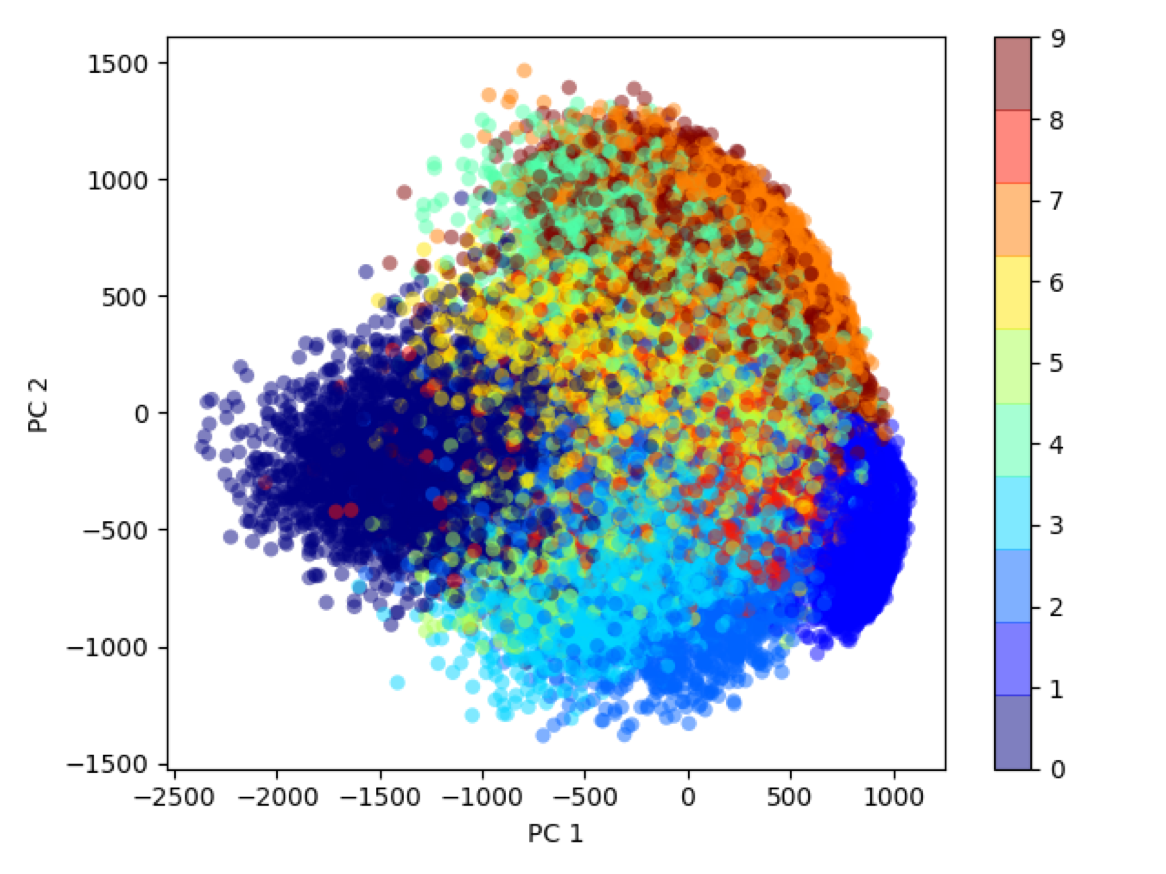
\includegraphics[width=\textwidth]{images/pca.png}
    \caption{PCA results}
    \setlength{\belowcaptionskip}{-20pt}
    \setlength{\abovecaptionskip}{-20pt}
\end{figure}


\section*{About k-Nearest Neighbor Algorithm}
\lipsum[1-1]

\begin{figure}[H]
    \centering
    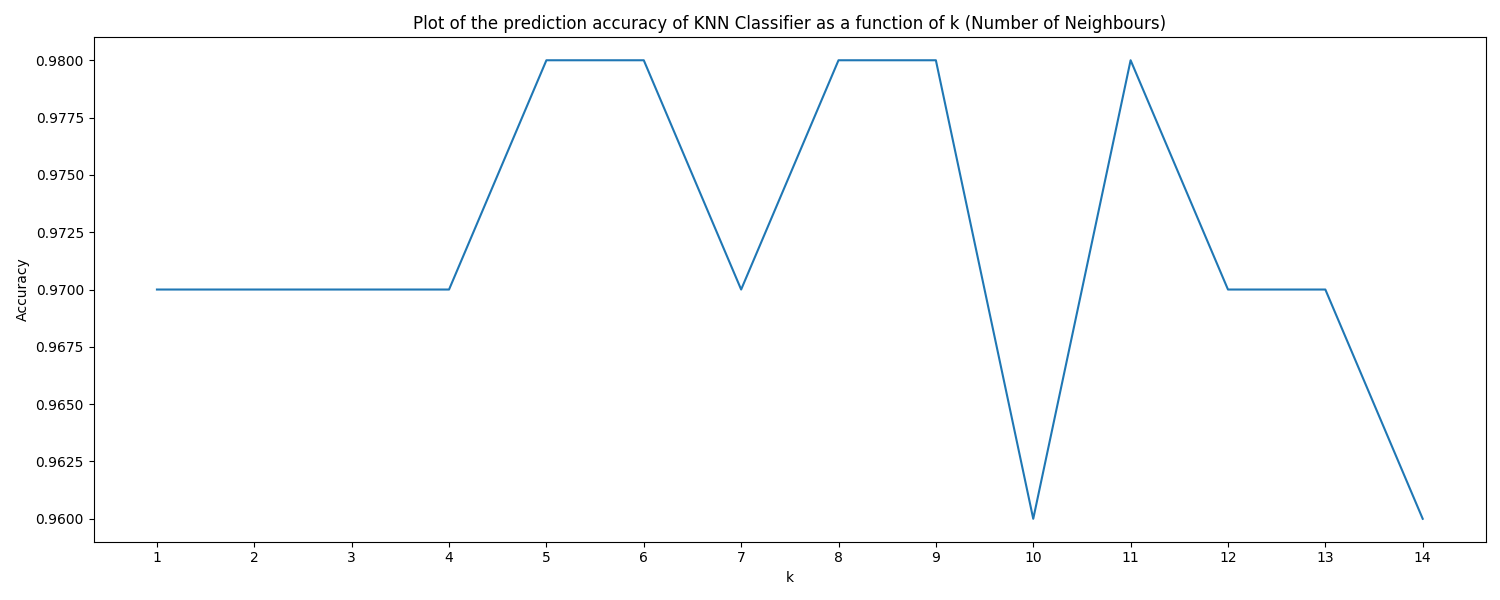
\includegraphics[width=\textwidth]{images/knn.png}
    \caption{k-Nearest Neighbor accuracy results}
    \setlength{\belowcaptionskip}{-20pt}
    \setlength{\abovecaptionskip}{-20pt}
\end{figure}

\lipsum[1-1]

\begin{table}[]
    \centering
    \begin{tabular}{llllllllllll}
        Actual & 0 & 1  & 2 & 3  & 4  & 5 & 6  & 7  & 8 & 9  & All \\
        0      & 8 & 0  & 0 & 0  & 0  & 0 & 0  & 0  & 0 & 0  & 8   \\
        1      & 0 & 14 & 0 & 0  & 0  & 0 & 0  & 0  & 0 & 0  & 14  \\
        2      & 0 & 0  & 7 & 1  & 0  & 0 & 0  & 0  & 0 & 0  & 8   \\
        3      & 0 & 0  & 0 & 11 & 0  & 0 & 0  & 0  & 0 & 0  & 11  \\
        4      & 0 & 0  & 0 & 0  & 13 & 0 & 0  & 0  & 0 & 1  & 14  \\
        5      & 0 & 0  & 1 & 0  & 0  & 6 & 0  & 0  & 0 & 0  & 7   \\
        6      & 0 & 0  & 0 & 0  & 0  & 0 & 10 & 0  & 0 & 0  & 0   \\
        7      & 0 & 0  & 0 & 0  & 0  & 0 & 0  & 15 & 0 & 0  & 15  \\
        8      & 0 & 0  & 0 & 0  & 0  & 0 & 0  & 0  & 2 & 0  & 2   \\
        9      & 0 & 0  & 0 & 0  & 0  & 0 & 0  & 0  & 0 & 11 & 11  \\
        All    & 8 & 14 & 8 & 12 & 13 & 6 & 10 & 15 & 2 & 12 & 100   
    \end{tabular}
    \caption*{Confusion Matrix of kNN classifier}
\end{table}

%\cite{watson_2020s}

\begin{lstlisting}[language=Python, caption=Caption for the snippet]
# Code snippet
print("I am a code snippet!")
\end{lstlisting}

%\newpage

\section*{Section Title}

\lipsum[1-3]

\section*{Section Title}
\lipsum[1-2]

